\documentclass[11pt,a4paper]{article}

% ---------------------------------------------------------------
% Packages
% ---------------------------------------------------------------
\usepackage[T1]{fontenc}
\usepackage{amsmath, amsthm, mathtools}
\usepackage{libertinus}
\usepackage{libertinust1math}
\usepackage{bm}
\usepackage{graphicx}
\usepackage{xcolor}
\usepackage{tikz}
\usetikzlibrary{arrows.meta, patterns}
\usepackage[most]{tcolorbox}
\usepackage{siunitx}
\sisetup{group-separator={\,}, group-minimum-digits=4, exponent-product=\cdot}
\DeclareSIUnit\angstrom{\text{\AA}}
\DeclareSIUnit\bohr{\ensuremath{a_0}}
\usepackage{booktabs}
\usepackage{tabularx}
\usepackage[numbers,sort&compress]{natbib}
\usepackage{microtype}
\usepackage{parskip}
\usepackage[margin=2.5cm, headheight=20pt]{geometry}
\usepackage{titlesec}
\usepackage{fancyhdr}
\usepackage{lastpage}
\usepackage{hyperref}
\usepackage[capitalise,noabbrev]{cleveref}

\numberwithin{equation}{section}

% ---------------------------------------------------------------
% Corporate colours (sampled from the FAU logo) and layout
% ---------------------------------------------------------------
\definecolor{faublue}{RGB}{0,47,108}
\definecolor{fautech}{RGB}{119,159,181}

\hypersetup{colorlinks=true, linkcolor=faublue, citecolor=faublue, urlcolor=faublue,
  pdftitle={The Phase-Field Method},
  pdfauthor={Ali Ghelichkhani}}

\titleformat{\section}{\sffamily\Large\bfseries\color{faublue}}{\thesection}{0.75em}{}
\titleformat{\subsection}{\sffamily\large\bfseries\color{faublue}}{\thesubsection}{0.7em}{}
\titleformat{\paragraph}[runin]{\sffamily\bfseries\color{faublue}}{}{0pt}{}
\titlespacing*{\paragraph}{0pt}{1.2ex plus 0.4ex}{0.6em}

\pagestyle{fancy}
\fancyhf{}
\fancyhead[L]{\sffamily\small\color{fautech}Materials Simulation Practical~5 \textbullet{} Part~I}
\fancyhead[R]{\raisebox{-0.2\height}{
\includegraphics[height=0.42cm]{figures/ww8.png}}}
\fancyfoot[L]{\sffamily\small\color{fautech}A.~Ghelichkhani}
\fancyfoot[R]{\sffamily\small\color{fautech}\thepage\ / \pageref*{LastPage}}
\renewcommand{\headrule}{\hbox to\headwidth{\color{fautech}\leaders\hrule height 0.4pt\hfill}}

\newtcolorbox{task}[1]{enhanced, sharp corners, frame hidden,
  colback=fautech!12, borderline west={2.5pt}{0pt}{faublue},
  left=9pt, right=9pt, top=6pt, bottom=6pt, after skip=12pt,
  before={\par\nopagebreak\vskip 6pt},
  fontupper=\sffamily\small,
  before upper={{\bfseries\color{faublue}Task~#1.}\enspace}}
\setcounter{MaxMatrixCols}{20}

\theoremstyle{remark}
\newtheorem{remark}{Remark}[section]

% ---------------------------------------------------------------
% Notation
% ---------------------------------------------------------------
\newcommand{\bigO}[1]{\mathcal{O}\!\left(#1\right)}
\newcommand{\fd}[2]{\frac{\delta #1}{\delta #2}}
\newcommand{\fb}{f_{\mathrm{bulk}}}
\newcommand{\fg}{f_{\mathrm{grad}}}
\newcommand{\cg}{c^{e}_{\gamma}}
\newcommand{\cgp}{c^{e}_{\gamma'}}
\newcommand{\bn}{\bm{n}}
\newcommand{\bu}{\bm{u}}

\begin{document}

\begin{titlepage}
  \noindent
  
\includegraphics[height=2.0cm]{figures/fau-techfak.png}\hfill
  \raisebox{0.6cm}{
\includegraphics[height=1.1cm]{figures/ww8.png}}

  \vspace{0.2cm}
  {\color{fautech}\rule{\textwidth}{0.6pt}}\\[0.1cm]
  {\sffamily\small\color{fautech}Institute of Materials Simulation (WW8)\hfill
    Winter semester 2026/27}

  \vspace*{3.4cm}
  {\sffamily\large\color{fautech}\textls[120]{MATERIALS SIMULATION PRACTICAL 5}\par}
  \vspace{0.5cm}
  {\sffamily\bfseries\color{faublue}\fontsize{30}{36}\selectfont
    The Phase-Field Method\par}
  \vspace{0.5cm}
  {\sffamily\Large\color{faublue}Free-Energy Functionals, Finite Volumes and the Ni--Al
    $\gamma/\gamma'$ Interface\par}
  \vspace{0.7cm}
  {\color{faublue}\rule{3cm}{2pt}}\par
  \vspace{0.4cm}
  {\sffamily\large Report, Part~I \textbullet{} Theory and Results\par}

  \vfill
  {\sffamily
  \renewcommand{\arraystretch}{1.35}
  \begin{tabular}{@{}>{\small\color{fautech}}l@{\hspace{1.2em}}l@{}}
    Author     & Ali Ghelichkhani \\
    E-mail     & \href{mailto:ali.ghelichkhani@fau.de}{ali.ghelichkhani@fau.de} \\
    Supervisor & Frank Wendler \\
    Module     & Foundations of Materials Simulation \\
    Institute  & Institute of Materials Simulation (WW8), FAU Erlangen-N\"urnberg \\
    Part~II    & Implementation, Jupyter notebook \texttt{phasefield.ipynb}
  \end{tabular}\par}
\end{titlepage}

\section*{Abstract}
  We review the three ingredients of a phase-field model --- order parameters, a free-energy
  functional, and gradient-flow kinetics --- and the finite volume method used to solve the resulting
  equations. For the symmetric double-well functional
  $F = \int f_0\phi^2(1-\phi)^2 + \tfrac{K_\phi}{2}|\nabla\phi|^2$ we derive the functional derivative,
  the equilibrium $\tanh$ profile of half-width $\delta = \sqrt{K_\phi/2f_0}$ and the interface energy
  $\sigma = \sqrt{2f_0K_\phi}/6$, and confirm all three with a one-dimensional Allen--Cahn simulation in
  FiPy: $f_0$ sharpens the interface, $K_\phi$ widens it, both raise its energy, and the mobility $L$
  affects only the kinetics. The simulated energy converges to the analytic value once the interface
  spans four to six control volumes, and the explicit scheme is stable only below $\Delta t = 0.5$. For
  the Ni--Al $\gamma/\gamma'$ system the barrier $\Delta f = \SI{149.9}{\joule\per\mole}$ gives a bulk
  coefficient $f_0 \approx \SI{1e8}{\joule\per\mole}$. A Cahn--Hilliard interface with
  $K_c = \SI{1e-7}{\joule\per\metre}$, the smallest value of the suggested range, has an energy of
  $\SI{81}{\milli\joule\per\metre\squared}$ and a width of $\SI{4}{\nano\metre}$; the experimental
  window of 5--50\,mJ/m$^2$ would require $K_c \approx 4\cdot10^{-10}$--$4\cdot10^{-8}$\,J/m, and in
  every case the prescribed \SI{10}{\nano\metre} grid is too coarse to resolve the interface. A 2D
  simulation from $c = 0.195$ shows spinodal decomposition into $\gamma$ and $\gamma'$ domains with a
  characteristic wavelength of $\SI{13}{\nano\metre}$, as linear stability theory predicts. The
  simulations are in the Jupyter notebook of Part~II; all their figures and results are included in
  this report.

\tableofcontents
\clearpage

% ===============================================================
\section{Introduction}\label{sec:intro}
% ===============================================================

Microstructure links processing to properties: the grains, phases and interfaces of a material are
set by its thermal and mechanical history, and they in turn set its strength, toughness and
conductivity. Following the evolution of a microstructure \emph{in situ} is rarely possible
experimentally, which is where simulation comes in. The phase-field method~\citep{script5,
chen2002, provatas2010} describes a microstructure by continuous fields that are constant inside each
phase or grain and vary smoothly across the interfaces between them. The interfaces are therefore
never tracked explicitly; their position, curvature and motion all follow from a single free-energy
functional and a gradient-flow equation. This makes it straightforward to handle topological changes
--- coalescence, splitting, the appearance of new domains --- that defeat sharp-interface methods.

This report covers the theory of the method (\cref{sec:model}), its finite volume discretization
(\cref{sec:fvm}) and three applications: single-component solidification in one dimension
(\cref{sec:task1}), the bulk energy coefficient of the Ni--Al $\gamma/\gamma'$ system
(\cref{sec:task2}), and the gradient energy coefficient together with a two-dimensional spinodal
decomposition (\cref{sec:task3}). The simulations are run in the Jupyter notebook of Part~II, and
their figures and results are presented in those sections.

\begin{table}[ht]
  \centering
  \caption{Correspondence between the tasks of the tutorial script and this report.}
  \label{tab:taskmap}
  \begin{tabularx}{0.9\linewidth}{lXl}
    \toprule
    Task & Content & Section \\
    \midrule
    Theory & order parameters, free energy, kinetics & \ref{sec:model} \\
    Theory & finite volume method: discretization, boundaries, assessment, explicit/implicit
           & \ref{sec:fvm} \\
    1 & 1D solidification: $\delta F/\delta\phi$, effect of $f_0$, $K_\phi$, $L$
      & \ref{sec:task1} (+ Part~II) \\
    2 & bulk energy coefficient $f_0$ for Ni--Al & \ref{sec:task2} (+ Part~II) \\
    3 & gradient energy coefficient $K_c$; 2D simulation & \ref{sec:task3} (+ Part~II) \\
    \bottomrule
  \end{tabularx}
\end{table}

% ===============================================================
\section{The phase-field model}\label{sec:model}
% ===============================================================

\subsection{Microstructure description}\label{sec:op}

A microstructure is described by one or more \emph{order parameters}: fields $\eta(\bm{r},t)$ that
take a constant value in each phase or grain and change continuously across the interface between
them, for example $\eta = 0$ in phase A, $\eta = 1$ in phase B and $0 < \eta < 1$ in a diffuse
interface of finite width $\lambda$. The field need not measure ``order'' in the crystallographic
sense: it can label a phase, a grain orientation, or the slipped and unslipped regions on either side
of a dislocation loop.

The decisive classification is whether the order parameter is \emph{conserved}. A
\emph{non-conserved} field, such as the solid fraction $\phi$ in the solidification of a pure
substance, can change locally without any compensating change elsewhere --- all of the liquid may
freeze. A \emph{conserved} field, such as the local composition $c$ in an alloy, can only be
redistributed: the total amount $\int c\,\mathrm{d}V$ is fixed, so it can change at a point only by a
flux into or out of it. The two cases lead to different kinetic equations (\cref{sec:kinetics}).

\subsection{Thermodynamics: the free-energy functional}\label{sec:thermo}

The total free energy is a functional of the fields,
\begin{equation}\label{eq:F}
  F = F_{\mathrm{bulk}} + F_{\mathrm{grad}} + F_{\mathrm{elas}} + \dots,
  \qquad
  F_{\mathrm{bulk}} + F_{\mathrm{grad}} = \int\left(\fb(c,\phi) + \frac{K_c}{2}|\nabla c|^2
    + \frac{K_\phi}{2}|\nabla\phi|^2\right)\mathrm{d}\bm{r}.
\end{equation}
The bulk term is the free energy of a homogeneous material of the local composition or phase. In the
simplest phenomenological (Landau) form for two phases it is a double well,
\begin{equation}\label{eq:dw}
  \fb = f_0\,\phi^2(1-\phi)^2,
\end{equation}
with minima of zero at the two pure phases and a barrier of height $\Delta f = f_0/16$ at
$\phi = 1/2$; the coefficient $f_0$ is fitted to $\Delta f$ taken from a thermodynamic assessment. The
gradient term accounts for the extra energy of an inhomogeneous region: across an interface $\phi$
takes intermediate values that the bulk term alone would assign too little energy to, and
$\tfrac{K}{2}|\nabla\phi|^2$ supplies the missing part. Together they define the interface energy, and
$K$ is chosen to reproduce its measured value. Further contributions --- elastic, plastic, magnetic,
electrostatic --- are added as the problem requires, for example
$f_{\mathrm{elas}} = \tfrac12 C_{ijkl}\varepsilon^{\mathrm{el}}_{ij}\varepsilon^{\mathrm{el}}_{kl}$.

\subsection{Kinetics}\label{sec:kinetics}

The fields evolve so as to lower $F$. The \emph{functional derivative} measures how $F$ changes with a
local variation of the field; for $F = \int f(\phi,\nabla\phi)\,\mathrm{d}\bm{r}$ it is
\begin{equation}\label{eq:fd}
  \fd{F}{\phi} = \frac{\partial f}{\partial\phi} - \nabla\cdot\frac{\partial f}{\partial(\nabla\phi)}.
\end{equation}
Non-conserved fields relax at a rate proportional to this driving force (Allen--Cahn), conserved
fields move by a flux proportional to its gradient (Cahn--Hilliard):
\begin{equation}\label{eq:ac-ch}
  \frac{\partial\phi}{\partial t} = -L\,\fd{F}{\phi},
  \qquad
  \frac{\partial c}{\partial t} = \nabla\cdot\left(M\nabla\fd{F}{c}\right).
\end{equation}
Both are gradient flows: inserting them into $\mathrm{d}F/\mathrm{d}t = \int(\delta F/\delta\phi)\,
\partial_t\phi$ gives $-L\int(\delta F/\delta\phi)^2 \le 0$ and
$-M\int|\nabla\,\delta F/\delta c|^2 \le 0$, so the free energy can only decrease and the evolution
stops at a stationary point $\delta F = 0$. Monitoring $F(t)$ during a simulation is therefore a
direct check on its correctness: an increasing $F$ signals a bug or an unstable scheme.

% ===============================================================
\section{The finite volume method}\label{sec:fvm}
% ===============================================================

\subsection{Discretization}\label{sec:fvdisc}

The finite volume method divides the domain into control volumes around the grid nodes $P$ and
integrates the general conservation equation
\begin{equation}\label{eq:general}
  \frac{\partial(\rho\phi)}{\partial t} = -\nabla\cdot(\bu\phi) + \nabla\cdot(\Gamma\nabla\phi) + S
\end{equation}
over each of them. The divergence theorem turns the convection and diffusion terms into fluxes through
the faces $g \in \{e,w,n,s\}$,
\begin{equation}\label{eq:fvint}
  \frac{(\rho\phi_P - \rho\phi_P^{\mathrm{old}})\Delta V}{\Delta t}
  = -\sum_g\phi_g(\bu\cdot\bn_g)A_g + \sum_g\Gamma(\nabla\phi\cdot\bn_g)_gA_g + (S_0 + S_1\phi_P)\Delta V.
\end{equation}
Face values are interpolated, $\phi_g = \alpha_g\phi_P + (1-\alpha_g)\phi_G$, and face gradients
approximated by $(\phi_G - \phi_P)/d_{GP}$, which turns \cref{eq:fvint} into the algebraic system
\begin{equation}\label{eq:aP}
  a_P\phi_P = \sum_G a_G\phi_G + b_P .
\end{equation}
Because the flux leaving one control volume through a face is by construction the flux entering its
neighbour, the method is \emph{conservative}: summed over the domain all interior fluxes cancel and
the total changes only through the boundary. This is the property that makes it the natural choice
for the Cahn--Hilliard equation, where the total composition must be preserved exactly. The source is
split into $S_0 + S_1\phi_P$ with $S_1 \le 0$, so that the $\phi$-dependent part of the source adds to
the diagonal $a_P$ and improves stability --- the device we use in \cref{sec:task1} for the
double-well source.

\subsection{Boundary conditions}\label{sec:fvbc}

In 1D with $I$ control volumes, \cref{eq:aP} has $I$ equations for $I+2$ unknowns, the two extra
ones belonging to virtual volumes outside the domain. They are eliminated with the boundary condition
$a\phi + b\nabla\phi\cdot\bn = \text{const}$: Dirichlet for $b = 0$, Neumann for $a = 0$, Robin
otherwise. The phase-field simulations of Part~II use zero-flux (homogeneous Neumann) boundaries in 1D,
which conserve the total of $c$ and do not pin the interface, and periodic boundaries in 2D, which
remove boundary effects altogether.

\subsection{Assessment: conservativeness, boundedness, transportiveness}\label{sec:fvassess}

A good scheme is conservative (\cref{sec:fvdisc}), bounded --- in the absence of sources the solution
stays between its boundary values, which the scaled diagonal dominance
$\sum|a_G|/|a_P| \le 1$ guarantees together with coefficients of one sign --- and transportive: it
respects the direction of information flow. Transportiveness is measured by the P\'eclet number
$Pe = C_g/D_g = \rho u\,d_{GP}/\Gamma$. Central differencing ($\alpha_g = 1/2$) is accurate for
$|Pe| < 2$ but produces negative coefficients and oscillations beyond; upwinding ($\alpha_g = 0$ or
$1$) is bounded for any $Pe$ but only first-order accurate; the hybrid scheme switches between the two
at $|Pe| = 2$. The phase-field equations of this practical contain no convection, $Pe = 0$, so central
differencing is exact in this respect and the issue does not arise.

\subsection{Explicit and implicit schemes}\label{sec:explicit}

If the neighbour values $\phi_G$ in \cref{eq:aP} are taken at the old time level, each $\phi_P$ is
computed directly from known quantities: the scheme is \emph{explicit}, cheap per step, but stable
only if all coefficients stay positive, which for diffusion requires
$\Delta t < \Delta x^2/(2\Gamma)$ in 1D (half that in 2D), and for the fourth-order Cahn--Hilliard
operator $\Delta t \propto \Delta x^4$. If they are taken at the new level, a linear system must be
solved per step: the scheme is \emph{implicit}, unconditionally stable for diffusion, but more
expensive per step. The simulations use both and illustrate the trade-off: FiPy's implicit solve runs the
Allen--Cahn problem at $\Delta t = 1$, whereas the explicit update fails beyond $\Delta t = 0.5$; for
the spinodal stage of the Cahn--Hilliard problem the explicit scheme is used and its step limited to
$\Delta t \approx 10^{-5}$\,s (\cref{sec:spinodal}).

% ===============================================================
\section{One-dimensional solidification (Task 1)}\label{sec:task1}
% ===============================================================

\begin{task}{1}
  A single component solidifies; $\phi = 0$ is liquid and $\phi = 1$ solid, with
  $F = \int f_0\phi^2(1-\phi)^2 + \tfrac{K_\phi}{2}|\nabla\phi|^2\,\mathrm{d}\bm{r}$ and
  $\partial_t\phi = -L\,\delta F/\delta\phi$. Write down $\delta F/\delta\phi$ analytically. With
  $f_0 = K_\phi = L = \Delta x = \Delta t = 1$, change $f_0$, $K_\phi$ and $L$ one at a time and
  describe their influence, plotting $\phi(x)$, $F(t)$ and the energy density field.
\end{task}

\subsection{Functional derivative and governing equation}\label{sec:derivative}

With $f = f_0\phi^2(1-\phi)^2 + \tfrac{K_\phi}{2}|\nabla\phi|^2$, \cref{eq:fd} has the two parts
\begin{equation}\label{eq:parts}
  \frac{\partial f}{\partial\phi} = 2f_0\,\phi(1-\phi)^2 - 2f_0\,\phi^2(1-\phi)
  = 2f_0\,\phi(1-\phi)(1-2\phi),
  \qquad
  \nabla\cdot\frac{\partial f}{\partial(\nabla\phi)} = \nabla\cdot(K_\phi\nabla\phi) = K_\phi\nabla^2\phi,
\end{equation}
so that
\begin{equation}\label{eq:dFdphi}
  \boxed{\;\fd{F}{\phi} = 2f_0\,\phi(1-\phi)(1-2\phi) - K_\phi\nabla^2\phi\;}
  \qquad\text{and}\qquad
  \frac{\partial\phi}{\partial t} = LK_\phi\nabla^2\phi - 2Lf_0\,\phi(1-\phi)(1-2\phi).
\end{equation}
The Allen--Cahn equation is a reaction--diffusion equation: the Laplacian smooths the profile, the
cubic reaction term drives $\phi$ towards the wells at 0 and 1.

\subsection{The equilibrium interface}\label{sec:eqprofile}

In one dimension the stationary state satisfies $K_\phi\phi'' = \partial\fb/\partial\phi$. Multiplying
by $\phi'$ and integrating once with $\phi' \to 0$ and $\fb \to 0$ far from the interface gives the
first integral
\begin{equation}\label{eq:firstint}
  \frac{K_\phi}{2}\,\phi'^2 = \fb(\phi) = f_0\phi^2(1-\phi)^2,
\end{equation}
which states that \emph{gradient and bulk energy densities are equal at every point of an equilibrium
interface}. Taking the root, $\phi' = \phi(1-\phi)/\delta$ with $\delta = \sqrt{K_\phi/2f_0}$, and
separating variables yields
\begin{equation}\label{eq:tanh}
  \phi(x) = \frac{1}{2}\left[1 + \tanh\frac{x}{2\delta}\right],
  \qquad
  \delta = \sqrt{\frac{K_\phi}{2f_0}},
  \qquad
  \lambda = \frac{1}{\max|\phi'|} = 4\delta .
\end{equation}
The interface energy is the excess energy per unit area,
\begin{equation}\label{eq:sigma}
  \sigma = \int_{-\infty}^{\infty}\left(\fb + \frac{K_\phi}{2}\phi'^2\right)\mathrm{d}x
  = \int K_\phi\phi'^2\,\mathrm{d}x = K_\phi\int_0^1\phi'\,\mathrm{d}\phi
  = \frac{K_\phi}{\delta}\int_0^1\phi(1-\phi)\,\mathrm{d}\phi
  = \frac{\sqrt{2f_0K_\phi}}{6},
\end{equation}
shared equally between the two contributions by \cref{eq:firstint}, $F_{\mathrm{bulk}} =
F_{\mathrm{grad}} = \sigma/2$. These three relations organize the whole parameter study.

\subsection{Simulation results}\label{sec:task1results}

The simulation starts from a sharp step on a 1D grid with $\Delta x = 1$ and relaxes it with FiPy. To run at the prescribed
$\Delta t = 1$, the reaction term is linearized about the old value and split into
$S_0 + S_1\phi$ with $S_1 = -L\,\partial^2\fb/\partial\phi^2$, the second part treated implicitly; a
fully explicit update is unstable for $\Delta t \ge 0.5$ (\cref{tab:explicit}).

\begin{table}[ht]
  \centering
  \caption{Stability of the explicit update for $f_0 = K_\phi = L = \Delta x = 1$. Both
    the diffusion limit $\Delta x^2/(2LK_\phi)$ and the reaction limit $1/(2Lf_0)$ equal $0.5$.}
  \label{tab:explicit}
  \begin{tabular}{lcccccc}
    \toprule
    $\Delta t$ & 0.10 & 0.25 & 0.40 & 0.50 & 0.60 & 1.00 \\
    \midrule
    explicit & stable & stable & stable & unstable & unstable & unstable \\
    $\max|\phi|$ & 1.000 & 1.000 & 1.103 & $1.0\times10^{6}$ & $1.5\times10^{9}$ & $1.5\times10^{4}$ \\
    \bottomrule
  \end{tabular}
\end{table}

\Cref{fig:ac1d} shows the result for the reference parameters $f_0 = K_\phi = L = 1$. The relaxed
profile coincides with \cref{eq:tanh} to within $0.018$ (left). The total energy reaches its plateau
after about ten time steps (centre): the gradient energy of the initial step falls while the bulk energy
rises, until the two meet at $F_{\mathrm{bulk}} = 0.1097$ and $F_{\mathrm{grad}} = 0.1092$, so
$F_{\mathrm{bulk}}/F_{\mathrm{grad}} = 1.004$ confirms the equipartition of \cref{eq:firstint}. The
energy density (right) is concentrated in the interface, where the bulk and the gradient contributions
have the same shape.

\begin{figure}[ht]
  \centering
  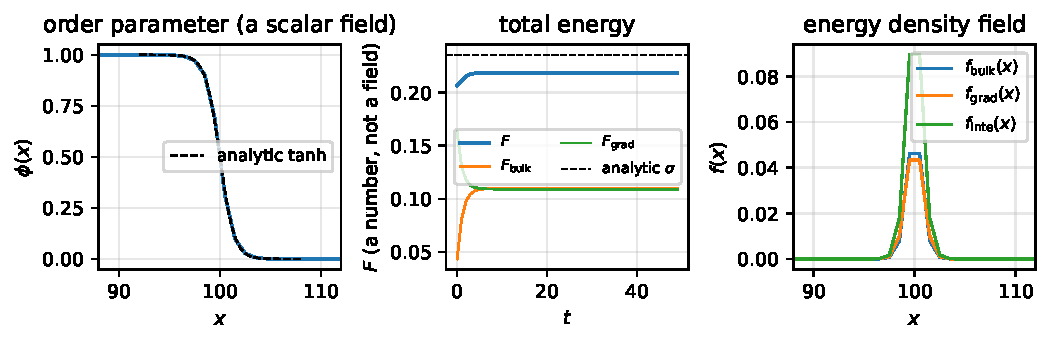
\includegraphics[width=\linewidth]{figures/fig_01.pdf}
  \caption{1D Allen--Cahn relaxation of a step with $f_0 = K_\phi = L = 1$. Left: final order
    parameter and the analytic $\tanh$ profile. Centre: total, bulk and gradient energy against time,
    with the analytic interface energy $\sigma$. Right: bulk, gradient and total energy density across
    the interface.}
  \label{fig:ac1d}
\end{figure} The plateau lies $7\,\%$ below the analytic
$\sigma = 0.2357$, because the interface is only $\lambda = 2.8$ cells wide and the discrete gradient
underestimates $|\nabla\phi|^2$. \Cref{tab:resolution} shows that the error disappears as $K_\phi$
widens the interface: four to six cells are needed for an error of one percent. On a logarithmic
scale the error falls almost linearly with the interface width (\cref{fig:resolution}).

\begin{figure}[ht]
  \centering
  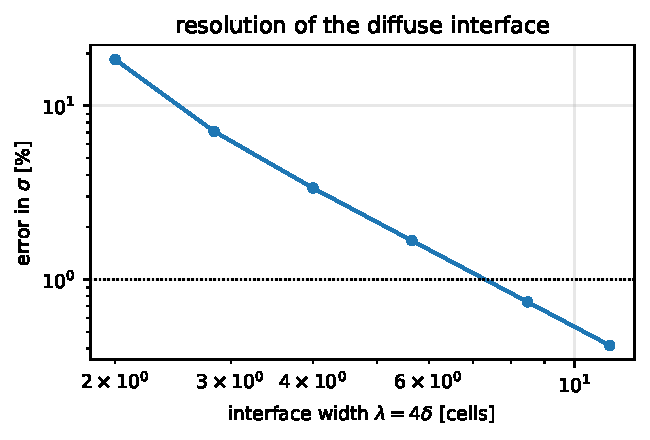
\includegraphics[width=0.55\linewidth]{figures/fig_03.pdf}
  \caption{Relative error of the simulated interface energy against the interface width
    $\lambda = 4\delta$ in grid cells; the dotted line marks $1\,\%$.}
  \label{fig:resolution}
\end{figure}

\begin{table}[ht]
  \centering
  \caption{Interface energy against resolution ($f_0 = 1$, $\Delta x = 1$).}
  \label{tab:resolution}
  \begin{tabular}{rrrrr}
    \toprule
    $K_\phi$ & $\lambda = 4\delta$ [cells] & $\sigma$ simulated & $\sigma$ analytic & error \\
    \midrule
    0.5  & 2.00  & 0.1359 & 0.1667 & 18.5\,\% \\
    1    & 2.83  & 0.2189 & 0.2357 & 7.1\,\% \\
    2    & 4.00  & 0.3221 & 0.3333 & 3.4\,\% \\
    4    & 5.66  & 0.4635 & 0.4714 & 1.7\,\% \\
    9    & 8.49  & 0.7019 & 0.7071 & 0.7\,\% \\
    16   & 11.31 & 0.9389 & 0.9428 & 0.4\,\% \\
    \bottomrule
  \end{tabular}
\end{table}

\paragraph{Influence of the coefficients.}
\Cref{fig:coeffs} shows the relaxed profiles for $f_0$ and $K_\phi$ between $0.25$ and $4$ and the
energy relaxation for three mobilities.
\begin{itemize}\setlength{\itemsep}{2pt}
  \item $f_0$ sets the height of the barrier between the two wells. Raising it penalizes intermediate
    $\phi$ and makes the interface \emph{thinner}, $\delta\propto f_0^{-1/2}$, and more energetic,
    $\sigma \propto f_0^{1/2}$. The measured interface width falls from 5.95 to 2.31 cells as $f_0$
    rises from $0.25$ to $4$. For $f_0 = 4$ the interface collapses to about two cells and the
    simulated $\sigma$ ($0.284$ against $0.471$) is $40\,\%$ too low --- a pure resolution artefact.
  \item $K_\phi$ penalizes gradients. Raising it makes the interface \emph{wider},
    $\delta\propto K_\phi^{1/2}$, and again more energetic, $\sigma\propto K_\phi^{1/2}$: the width rises
    from 2.31 to 5.95 cells and $\sigma$ from $0.071$ to $0.464$. Since it widens the interface it also
    improves the resolution.
  \item $L$ appears only in the time derivative. The equilibrium profile and energy are identical for
    $L = 0.1$, $0.5$ and $2$ (width 3.40 cells, $F = 0.2189$); only the time to reach them scales as
    $1/L$ (right panel of \cref{fig:coeffs}).
\end{itemize}

\begin{figure}[ht]
  \centering
  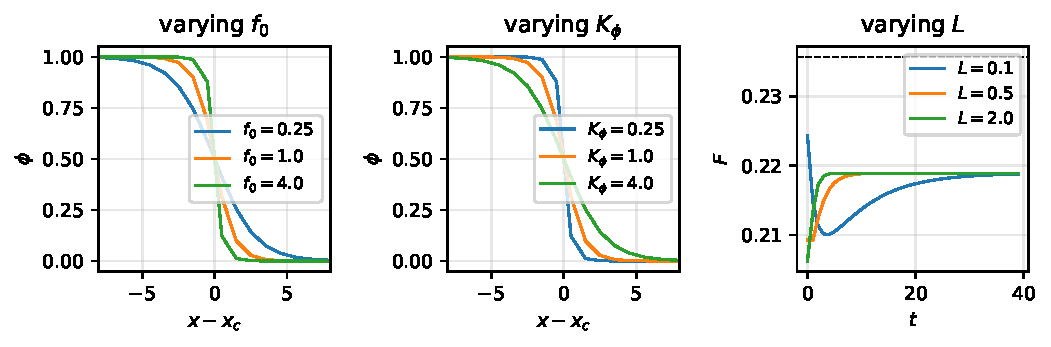
\includegraphics[width=\linewidth]{figures/fig_02.pdf}
  \caption{Influence of the coefficients of the Allen--Cahn model. Left and centre: relaxed profiles
    for $f_0$ and $K_\phi$ of $0.25$, $1$ and $4$ (the other coefficients equal to one). Right: total
    energy against time for three mobilities $L$; the dashed line is the analytic $\sigma$ for
    $f_0 = K_\phi = 1$.}
  \label{fig:coeffs}
\end{figure}
$f_0$ is therefore fixed by thermodynamics, $K_\phi$ is the free parameter that sets the interface
energy, and $L$ is fitted to kinetic data such as interface velocities.

\paragraph{Why the interface does not move.}
The double well \cref{eq:dw} is symmetric: solid and liquid have the same free energy, so there is no
driving force and the flat interface comes to rest after relaxing its shape. Real solidification
requires undercooling, which tilts the double well by a free-energy difference $\Delta f$ between the
phases; the interface then moves with a velocity proportional to $L\,\delta\,\Delta f$. A curved
interface would move even without a tilt, by the Gibbs--Thomson effect, at a velocity
$\propto L\sigma\kappa$.

% ===============================================================
\section{The bulk energy coefficient of Ni--Al (Task 2)}\label{sec:task2}
% ===============================================================

\begin{task}{2}
  For the Ni--Al system with the phases $\gamma$ and $\gamma'$ at 1300\,K the bulk energy density
  has a barrier $\Delta f = \SI{149.9}{\joule\per\mole}$ between the equilibrium compositions
  $\cg$ and $\cgp$. With $\fb = f_0(\cgp - c)^2(c - \cg)^2$, determine the rough value of $f_0$.
\end{task}

The polynomial vanishes at the two equilibrium compositions and, by symmetry, peaks halfway between
them at $c^* = (\cg + \cgp)/2$, where both factors equal $\Delta c/2$ with $\Delta c = \cgp - \cg$:
\begin{equation}\label{eq:f0}
  \Delta f = f_0\left(\frac{\Delta c}{2}\right)^4
  \qquad\Longrightarrow\qquad
  f_0 = \frac{\Delta f}{(\Delta c/2)^4}.
\end{equation}
Reading the minima from the figure of the script as $\cg = 0.16$ and $\cgp = 0.23$ gives
$\Delta c/2 = 0.035$ and
\begin{equation}\label{eq:f0value}
  \boxed{\;f_0 = \frac{\SI{149.9}{\joule\per\mole}}{(0.035)^4} = \SI{9.99e7}{\joule\per\mole}
  \approx \SI{1e8}{\joule\per\mole},\;}
  \qquad
  f_{0,V} = \frac{f_0}{V_m} \approx \SI{1e13}{\joule\per\metre\cubed}
\end{equation}
with $V_m = \SI{1e-5}{\cubic\metre\per\mole}$. The fourth power makes $f_0$ sensitive to how the minima
are read off: shifting one of them by $\pm0.005$ changes $f_0$ by about $30\,\%$
(\cref{tab:f0sens}), so only the order of magnitude is meaningful --- which is all a phenomenological fit can claim anyway. The large
number reflects the narrow two-phase field: a barrier of only $\SI{150}{\joule\per\mole}$ is built up
over a composition difference of $0.07$. \Cref{fig:nial} shows the resulting bulk energy density.

\begin{figure}[ht]
  \centering
  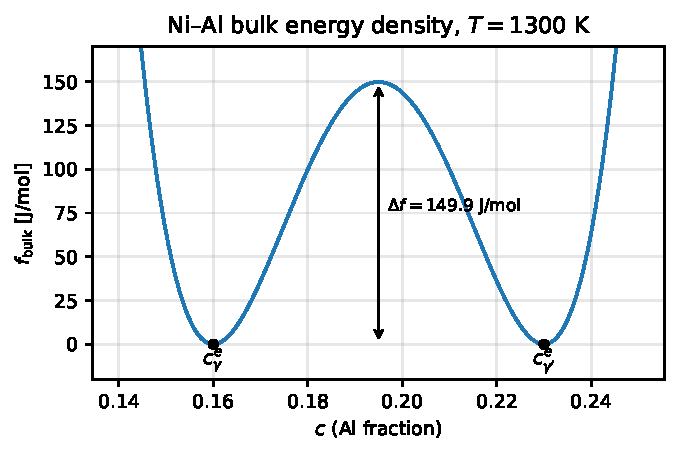
\includegraphics[width=0.6\linewidth]{figures/fig_04.pdf}
  \caption{Bulk energy density $f_0(\cgp - c)^2(c - \cg)^2$ of Ni--Al at 1300\,K with
    $f_0 = \SI{9.99e7}{\joule\per\mole}$, $\cg = 0.16$ and $\cgp = 0.23$. The barrier at
    $c = 0.195$ is $\Delta f = \SI{149.9}{\joule\per\mole}$.}
  \label{fig:nial}
\end{figure}

\begin{table}[ht]
  \centering
  \caption{Sensitivity of $f_0$ to the equilibrium compositions read off the figure of the script.}
  \label{tab:f0sens}
  \begin{tabular}{ccc}
    \toprule
    $\cg$ & $\cgp$ & $f_0$ [J/mol] \\
    \midrule
    0.160 & 0.225 & $1.34\times10^{8}$ \\
    0.160 & 0.230 & $9.99\times10^{7}$ \\
    0.160 & 0.235 & $7.58\times10^{7}$ \\
    0.155 & 0.230 & $7.58\times10^{7}$ \\
    \bottomrule
  \end{tabular}
\end{table}

% ===============================================================
\section{The gradient energy coefficient (Task 3)}\label{sec:task3}
% ===============================================================

\begin{task}{3}
  With $\fg = \tfrac{K_c}{2}|\nabla c|^2$ and $\partial_t c = M\nabla^2\,\delta F/\delta c$, and
  $V_m = \SI{1e-5}{\cubic\metre\per\mole}$,
  $M = \SI{1e-17}{\mole\squared\per\joule\per\metre\per\second}$, $\Delta t = \SI{1}{\second}$,
  $\Delta x = \SI{1e-8}{\metre}$ and an experimental interface energy of 5--50\,mJ/m$^2$, find a proper
  $K_c$ in the range $10^{-7}$--$10^{-4}$\,J/m with a 1D simulation, showing the numerical interface
  energy and thickness. Extend the simulation to 2D with $c = 0.195$ plus Gaussian noise and plot the
  field after $1000\,\Delta t$.
\end{task}

\subsection{Units and the governing equation}\label{sec:units}

The bulk energy is given per mole and $K_c$ in J/m, i.e.\ per unit volume, so the functional is
written per unit volume, $F_V = \int(\fb/V_m + \tfrac{K_c}{2}|\nabla c|^2)\,\mathrm{d}V$. The mobility in
mol$^2$/(J\,m\,s) relates a molar flux to the gradient of a molar chemical potential; converting both to
volumetric quantities with $c$ a mole fraction gives
\begin{equation}\label{eq:chunits}
  \frac{\partial c}{\partial t} = MV_m^2\,\nabla^2\fd{F_V}{c},
  \qquad
  \fd{F_V}{c} = \frac{1}{V_m}\frac{\partial\fb}{\partial c} - K_c\nabla^2c,
\end{equation}
with $MV_m^2 = \SI{1e-27}{\metre\tothe{5}\per\joule\per\second}$. With these values the characteristic
relaxation time of an interface is $\delta^4/(MV_m^2K_c)$, of the order of one second for an interface about as wide as the
prescribed grid spacing of \SI{10}{\nano\metre}, consistent with the prescribed $\Delta t = 1$\,s.

\subsection{Interface energy and width}\label{sec:kc}

The substitution $u = (c - \cg)/\Delta c$ maps the Ni--Al double well onto the symmetric form of
\cref{sec:task1} with effective coefficients $f_{0,V}\Delta c^4$ and $K_c\Delta c^2$, so
\cref{eq:tanh,eq:sigma} give
\begin{equation}\label{eq:kcrel}
  \delta = \frac{1}{\Delta c}\sqrt{\frac{K_c}{2f_{0,V}}},
  \qquad
  \sigma = \frac{\Delta c^3\sqrt{2f_{0,V}K_c}}{6}.
\end{equation}
\Cref{tab:kc} evaluates them and compares with 1D Cahn--Hilliard simulations, which reproduce $\sigma$
to $0.4\,\%$ with $F_{\mathrm{bulk}} = F_{\mathrm{grad}}$ to better than $2\,\%$ on a grid with
$\Delta x = \delta/3$. \Cref{fig:kc} shows the simulated profile for the chosen $K_c$ and the interface
energy over the whole range of $K_c$ together with the experimental window.

\begin{table}[ht]
  \centering
  \caption{Interface energy and half-width of the $\gamma/\gamma'$ interface as functions of $K_c$.
    The simulated values use $\Delta x = \delta/3$; the last column gives $\delta$ in units of
    the grid spacing $\Delta x = \SI{10}{\nano\metre}$ prescribed in the script.}
  \label{tab:kc}
  \begin{tabular}{rrrrr}
    \toprule
    $K_c$ [J/m] & $\sigma$ analytic [mJ/m$^2$] & $\sigma$ simulated [mJ/m$^2$] & $\delta$ [nm]
      & $\delta/(\SI{10}{\nano\metre})$ \\
    \midrule
    $10^{-9}$ & 8.1    & ---    & 0.10 & 0.01 \\
    $10^{-8}$ & 25.6   & ---    & 0.32 & 0.03 \\
    $10^{-7}$ & 80.8   & 80.5   & 1.01 & 0.10 \\
    $10^{-6}$ & 255.5  & 254.6  & 3.20 & 0.32 \\
    $10^{-5}$ & 808.0  & 805.1  & 10.1 & 1.01 \\
    $10^{-4}$ & 2555   & 2546   & 32.0 & 3.20 \\
    \bottomrule
  \end{tabular}
\end{table}

Two requirements conflict. Matching the measured interface energy of 5--50\,mJ/m$^2$ requires
$K_c = \SI{3.8e-10}{}$--$\SI{3.8e-8}{\joule\per\metre}$; resolving the interface with at least a few
cells of the prescribed \SI{10}{\nano\metre} grid requires $K_c \gtrsim \SI{1e-5}{\joule\per\metre}$,
which puts the interface energy at $\SI{800}{\milli\joule\per\metre\squared}$. The physical
$\gamma/\gamma'$ interface is about a nanometre wide, and a \SI{10}{\nano\metre} grid cannot carry it.
There are two standard ways out: refine the grid until $\Delta x \lesssim \delta$, or keep the coarse
grid and widen the interface artificially by raising $K_c$ and lowering $f_{0,V}$ together, which keeps
$\sigma\propto\sqrt{f_{0,V}K_c}$ fixed while $\delta\propto\sqrt{K_c/f_{0,V}}$ grows --- the
thin-interface rescaling of production codes.

\paragraph{Result.}
We choose the smallest value of the suggested range,
\begin{equation}\label{eq:kcchosen}
  \boxed{\;K_c = \SI{1e-7}{\joule\per\metre}:\qquad
  \sigma = \SI{81}{\milli\joule\per\metre\squared},\qquad
  \lambda = 4\delta = \SI{4.0}{\nano\metre},\;}
\end{equation}
on a refined grid with twelve cells across the interface. It is the value of the range closest to the
experimental window, a factor 1.6 above its upper end; hitting the middle of the window
($\approx\SI{25}{\milli\joule\per\metre\squared}$) would require $K_c\approx\SI{1e-8}{\joule\per\metre}$,
an order of magnitude below the suggested range. Since $\sigma\propto\Delta c^3\sqrt{f_0}$ and $f_0$
itself is uncertain by about $30\,\%$ (\cref{sec:task2}), this discrepancy is within the accuracy of
the input data.

\begin{figure}[ht]
  \centering
  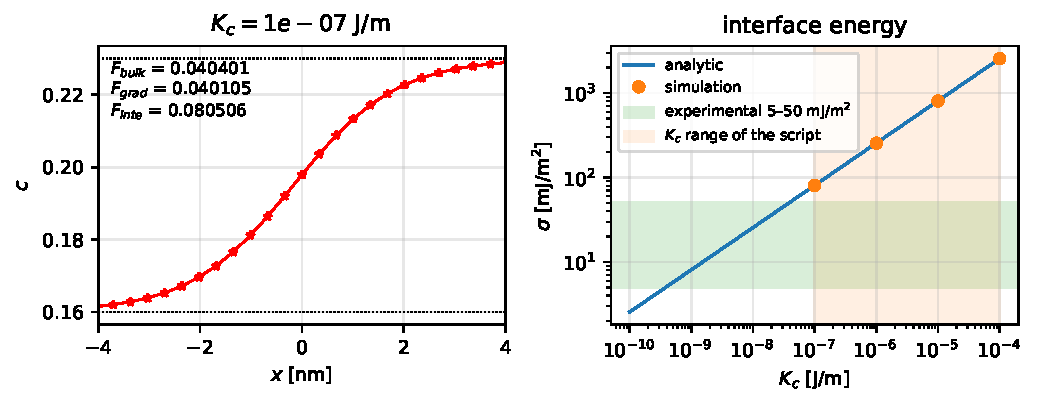
\includegraphics[width=\linewidth]{figures/fig_05.pdf}
  \caption{Left: equilibrium $\gamma/\gamma'$ composition profile from a 1D Cahn--Hilliard simulation
    with $K_c = \SI{1e-7}{\joule\per\metre}$ (markers: grid points, $\Delta x = \SI{0.337}{\nano\metre}$;
    dotted lines: equilibrium compositions), with the bulk, gradient and total interface energies in
    J/m$^2$. Right: interface energy against $K_c$ from \cref{eq:kcrel} and from the simulations, with
    the experimental window (green) and the range of $K_c$ suggested by the script (orange).}
  \label{fig:kc}
\end{figure}

\subsection{Spinodal decomposition in two dimensions}\label{sec:spinodal}

Starting the 2D simulation at $c = 0.195$, the top of the barrier, places the alloy inside the
spinodal, where $\partial^2\fb/\partial c^2 < 0$. Linearizing \cref{eq:chunits} about the uniform state
gives for a perturbation $\propto e^{i\bm{k}\cdot\bm{r} + R t}$ the growth rate
\begin{equation}\label{eq:growth}
  R(k) = -MV_m^2\,k^2\left(\frac{1}{V_m}\frac{\partial^2\fb}{\partial c^2} + K_ck^2\right),
\end{equation}
positive for wave numbers below $k_c = \sqrt{-\fb''/(V_mK_c)}$ and largest at $k_{\max} = k_c/\sqrt2$.
The uniform alloy is unstable: material diffuses \emph{up} the concentration gradient, a negative
effective diffusion coefficient that the gradient energy limits at short wavelengths. For
$K_c = \SI{1e-7}{\joule\per\metre}$ the fastest-growing wavelength is
$2\pi/k_{\max} = \SI{12.7}{\nano\metre}$ and its growth rate $R = \SI{6.0}{\per\second}$.

The simulation runs on a $\SI{64.7}{\nano\metre}\times\SI{64.7}{\nano\metre}$ periodic domain with
$\Delta x = \SI{0.505}{\nano\metre}$ and $\Delta t = \SI{1.3e-5}{\second}$, i.e.\ \num{153331} steps to
$t = \SI{2}{\second}$. \Cref{fig:spinodal} shows the expected sequence. The white noise of the initial
state first decays at short wavelengths; at $t = \SI{0.5}{\second}$ a faint pattern with a wavelength of
about $\SI{13}{\nano\metre}$ has emerged. It is amplified into an interconnected labyrinth of $\gamma$-
and $\gamma'$-rich domains, whose compositions at $\SI{2}{\second}$ span $0.159$ to $0.230$, i.e.\ the
equilibrium values $0.16$ and $0.23$. The mean composition is conserved ($0.195$ at the start,
$0.195012$ at the end). The free energy decreases monotonically: a short initial drop as the noise is
smoothed, a plateau while the unstable modes are still small, a steep fall around
$t \approx \SI{1}{\second}$ when the domains form, and a slower decrease as they start to coarsen.

\begin{figure}[ht]
  \centering
  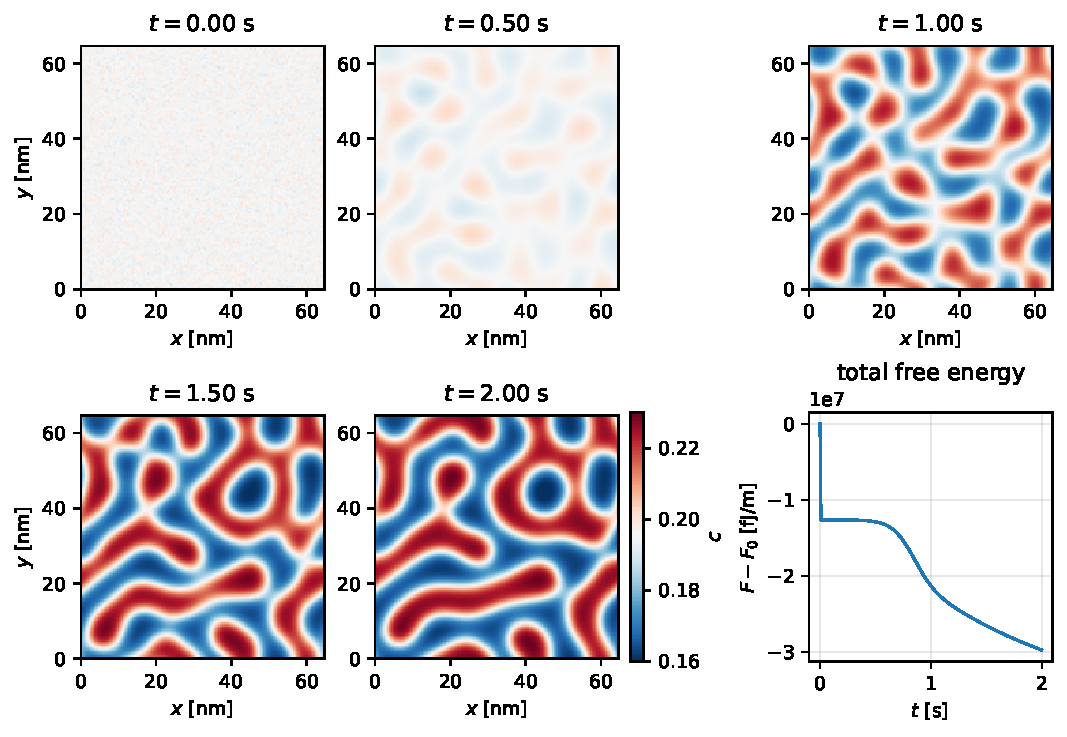
\includegraphics[width=\linewidth]{figures/fig_06.pdf}
  \caption{Spinodal decomposition of Ni--Al from $c = 0.195$ with small random noise on a
    $\SI{64.7}{\nano\metre}\times\SI{64.7}{\nano\metre}$ periodic domain. Five snapshots of the
    composition between $t = 0$ and $\SI{2}{\second}$ and the change of the total free energy.}
  \label{fig:spinodal}
\end{figure} Two numerical remarks apply. First, the FiPy formulation used for the 1D interface froze
at the initial noise level once the coefficient $\partial^2\fb/\partial c^2$ became negative, while an
explicit finite volume update of the same equation decomposed as \cref{eq:growth} predicts; the 2D run
therefore uses the explicit scheme. Second, the explicit step is limited by the fourth-order term to
$\Delta t\approx\SI{1.3e-5}{\second}$, so the prescribed ``$1000\,\Delta t$'' with $\Delta t = 1$\,s is
not reachable step by step; the snapshots are reported at physical times up to $\SI{2}{\second}$, which
covers the whole decomposition stage.

In a Ni-based superalloy this is the mechanism behind fine $\gamma'$ precipitation: with $f_0$ from
thermodynamics and $K_c$ from the interface energy, the model reproduces both the length scale of the
microstructure and its evolution.

% ===============================================================
\section{Conclusion}\label{sec:conclusion}
% ===============================================================

A phase-field model is defined by its free-energy functional: the bulk term sets which phases exist and
how stable they are, the gradient term sets the energy and the width of the interfaces between them, and
a gradient-flow equation --- Allen--Cahn for non-conserved, Cahn--Hilliard for conserved fields ---
lowers the energy monotonically. For the double well
$f_0\phi^2(1-\phi)^2 + \tfrac{K_\phi}{2}|\nabla\phi|^2$ the equilibrium interface is a $\tanh$ of
half-width $\sqrt{K_\phi/2f_0}$ with energy $\sqrt{2f_0K_\phi}/6$, split equally between bulk and
gradient contributions. The 1D solidification simulation confirms these results and shows the practical
roles of the coefficients: $f_0$ and $K_\phi$ together fix interface width and energy, $L$ only the time
scale, and the interface must span four to six control volumes for its energy to be computed to a
percent. For Ni--Al, the thermodynamic barrier fixes $f_0\approx\SI{1e8}{\joule\per\mole}$, and
$K_c = \SI{1e-7}{\joule\per\metre}$ gives an interface energy of $\SI{81}{\milli\joule\per\metre\squared}$
and a width of $\SI{4}{\nano\metre}$ --- of the right order, and a reminder that the physical interface
of this alloy is far finer than a \SI{10}{\nano\metre} grid can carry. The same model in 2D produces the
spinodal $\gamma/\gamma'$ microstructure with the wavelength predicted by linear stability theory.

\begin{thebibliography}{99}

\bibitem{script5}
Institute of Materials Simulation (WW8),
``Phase-field method: basics and application in materials science,''
Materials Simulation Practical No.~5, tutorial script,
Friedrich-Alexander-Universit\"at Erlangen-N\"urnberg.

\bibitem{chen2002}
L.-Q.~Chen,
``Phase-field models for microstructure evolution,''
\textit{Annual Review of Materials Research},
vol.~32, pp.~113--140, 2002.

\bibitem{provatas2010}
N.~Provatas and K.~Elder,
\textit{Phase-Field Methods in Materials Science and Engineering},
Wiley-VCH, Weinheim, 2010.

\bibitem{cahn1958}
J.~W.~Cahn and J.~E.~Hilliard,
``Free energy of a nonuniform system.~I.~Interfacial free energy,''
\textit{The Journal of Chemical Physics},
vol.~28, no.~2, pp.~258--267, 1958.

\bibitem{allen1979}
S.~M.~Allen and J.~W.~Cahn,
``A microscopic theory for antiphase boundary motion and its application to antiphase domain
coarsening,''
\textit{Acta Metallurgica},
vol.~27, no.~6, pp.~1085--1095, 1979.

\bibitem{guyer2009}
J.~E.~Guyer, D.~Wheeler and J.~A.~Warren,
``FiPy: Partial differential equations with Python,''
\textit{Computing in Science \& Engineering},
vol.~11, no.~3, pp.~6--15, 2009.

\bibitem{lesar2013}
R.~LeSar,
\textit{Introduction to Computational Materials Science: Fundamentals to Applications},
Cambridge University Press, Cambridge, 2013.

\bibitem{versteeg2007}
H.~K.~Versteeg and W.~Malalasekera,
\textit{An Introduction to Computational Fluid Dynamics: The Finite Volume Method},
2nd~ed., Pearson, Harlow, 2007.

\end{thebibliography}

\end{document}
